Se genera una señal de 2 tonos puros de 100 y 500 Hz con amplitudes $0,5$ y $1,5$ respectivamente. Se le agrega a esta señal ruido blanco de distribución normal de media 0 y varianza 2, muestreando la señal resultante durante 100 ms a $f_s = 2000~Hz$ para cumplir con el criterio de Nyquist.

En la figura \ref{fig:p2_1t} se muestra la representación temporal de la señal con ruido. A partir del gráfico no es posible reconocer que la señal limpia corresponde a la superposición de 2 tonos puros ni las frecuencias de estos.

\begin{figure}[H]
    \centering
    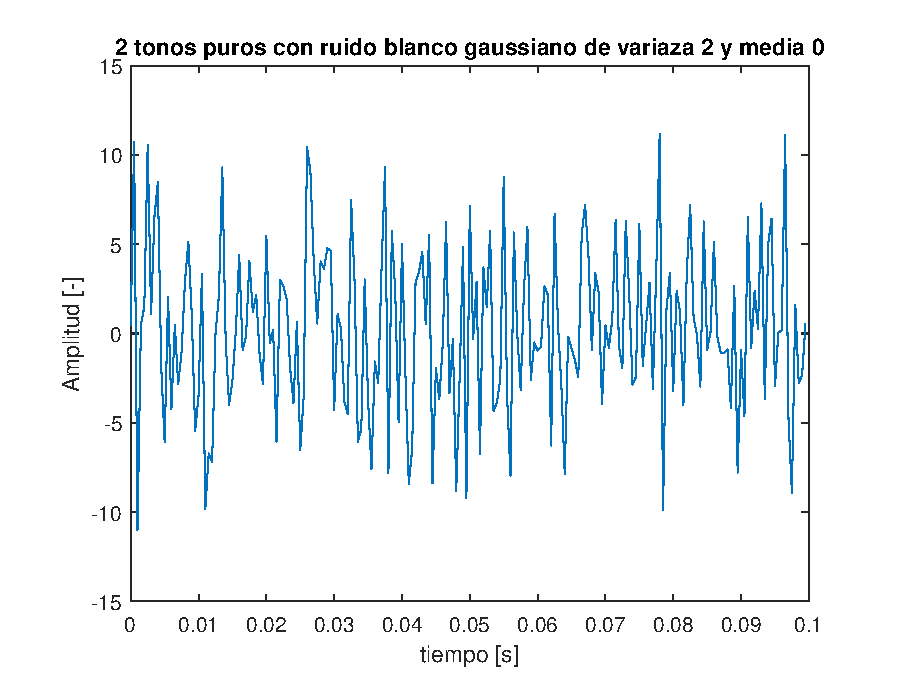
\includegraphics[width = .8\linewidth]{Figuras/1.eps}
    \caption{Representación temporal de señal de 2 tonos puros con ruido}
    \label{fig:p2_1t}
\end{figure}

Luego se grafica la magnitud del espectro de las señales con y sin ruido usando el comando $fft()$ de MATLAB. Dichos gráficos se muestran en la figura \ref{fig:p2_2mag} 

\begin{figure}[H]
    \centering
    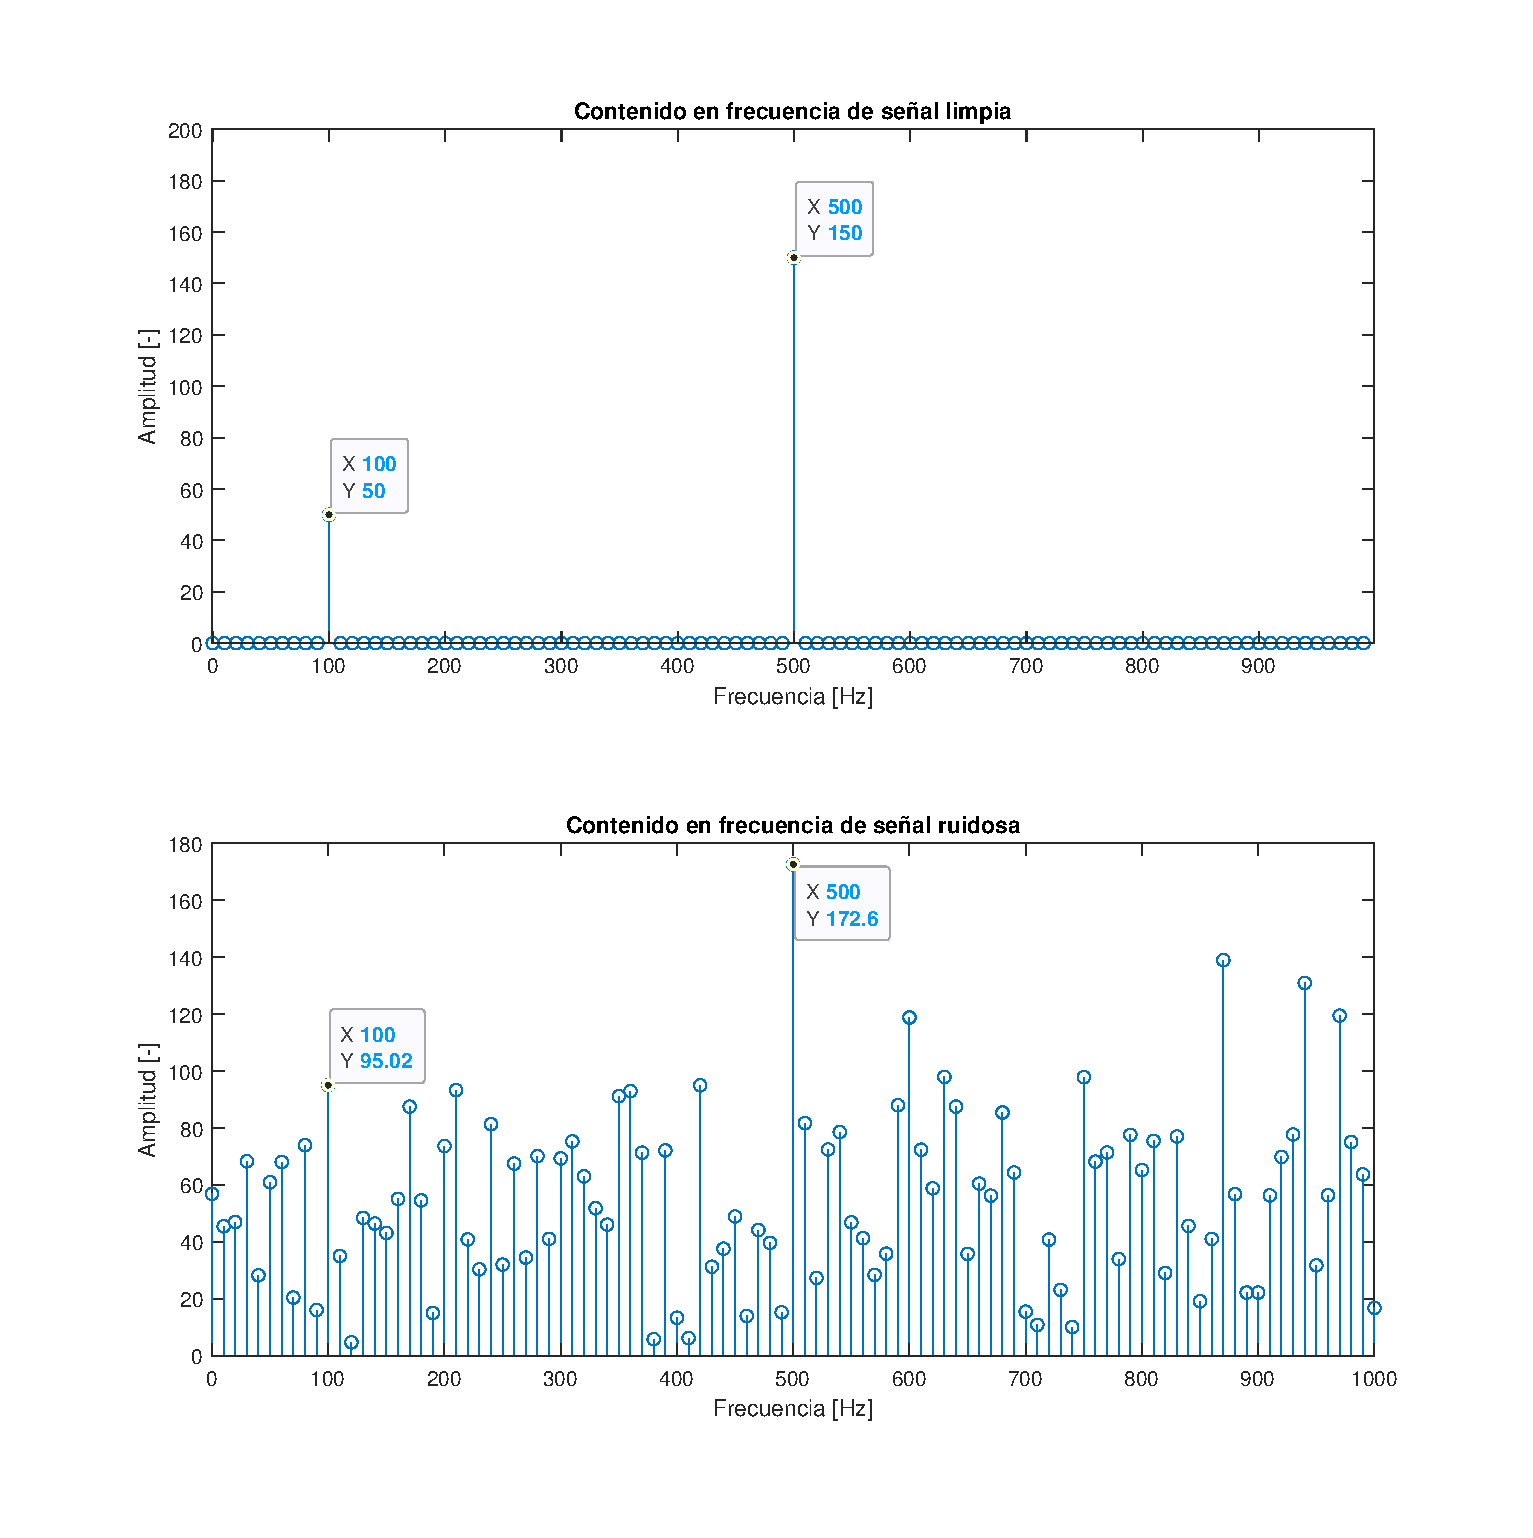
\includegraphics[width = .8\linewidth]{Figuras/2.eps}
    \caption{Magnitud del espectro de señal de 2 tonos puros sin y con ruido.}
    \label{fig:p2_2mag}
\end{figure}

Con respecto a la figura \ref{fig:p2_2mag} se aprecia que la amplitud de los tonos puros no es la misma en ambos casos. Lo anterior se debe a que el ruido agregado también tiene contenido en frecuencia en las frecuencias de los tonos puros.

Posteriormente se grafica la magnitud en dB del espectro en frecuencia de las señales con y sin ruido, normalizando la amplitud máxima a 0 dB. Dicho gráfico se muestra en la figura \ref{fig:p2_3mag}. En el caso de la señal limpia se observa que la diferencia de amplitud entre la componenente más elevada y el piso de ruido es de -300 dB aproximadamente. En el caso de la señal ruidosa es de aproximadamente -10 dB. 

\begin{figure}[H]
    \centering
    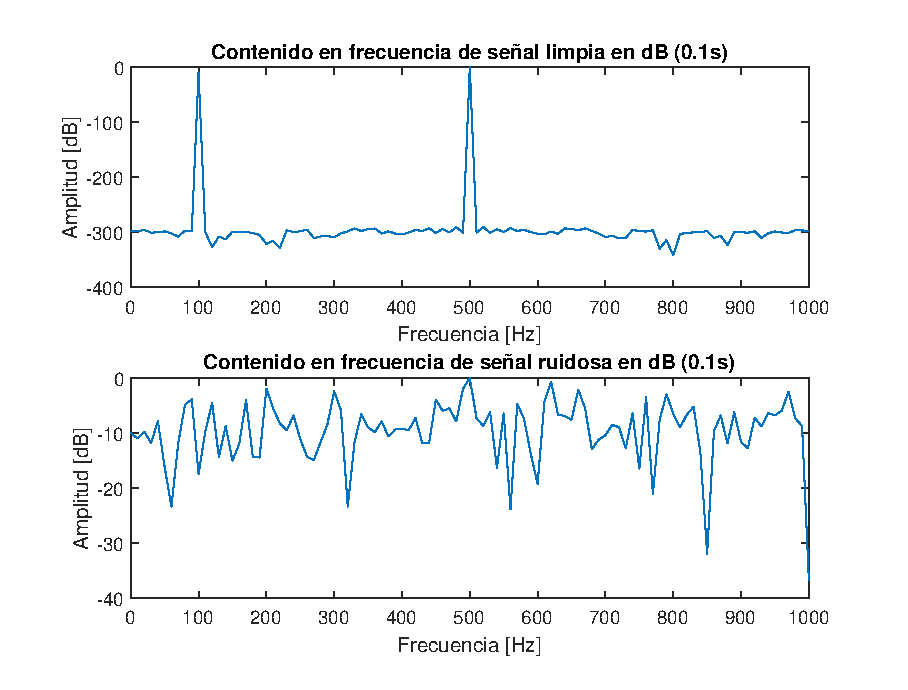
\includegraphics[width = .8\linewidth]{Figuras/3.eps}
    \caption{Magnitud en decibeles del espectro de señal de 2 tonos puros sin y con ruido, de duración 1 ms.}
    \label{fig:p2_3mag}
\end{figure}

%cCOMENTARIOS AMPLITUD

Finalmente se cambia la duración de la señal a 1s y se vuelve a graficar la magnitud normalizada en dB del espectro en frecuencia de las señales con y sin ruido. Dicho gráfico se muestra en la figura \ref{fig:p2_4mag}. Las diferencias entre el espectro encontrado con una ventana de 1 s y 0.1 s se debe a que la ventana de mayor largo en frecuencia es más angosta, lo que se traduce en un menor \textit{leakage}.

\begin{figure}[H]
    \centering
    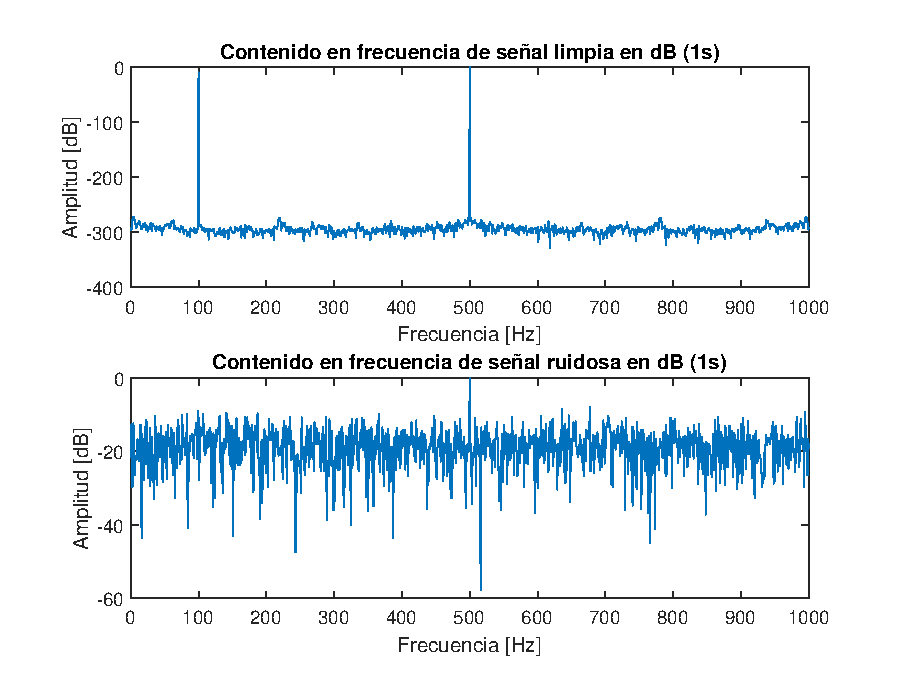
\includegraphics[width = .8\linewidth]{Figuras/4.eps}
    \caption{Magnitud en decibeles del espectro de señal de 2 tonos puros sin y con ruido, de duración 1 s.}
    \label{fig:p2_4mag}
\end{figure}